\FloatBarrier
\section{Microarchitecture}\label{sec:micro}

\subsection{The Atmospheric Vector Tile}
An AVT is deliberately narrow and deep. It holds 256 lanes in a 16$\times$16 array, each lane with
a 32-bit $\times$ 8 register slice, a 4-way SIMD FMA, a special-function unit shared by four lanes,
and a Kahan accumulator for reduction. Three time levels of the tile's 910-cell block live in
256 KB of SRAM; a 32 KB register file holds coefficients, halo edges and the current wavefront.

The pipeline has six stages: fetch, decode, issue, FMA, memory and write-back. Decode is 4-wide
and static: there is no branch predictor because the ISA has no branches, and no cache because
all addresses are compile-time constants within a tile's block. Issue is in-order with a
scoreboard that tracks the six-cycle SRAM latency and the sixteen-cycle SFU latency. The compiler
interleaves independent variable streams so that a dependent stall occurs roughly once per
sixteen vector operations; the modelled pipeline efficiency is 79.1\% on the advection kernel and
69.8\% on radiation, where SFU latency is harder to hide.

\begin{figure}[t]
\centering
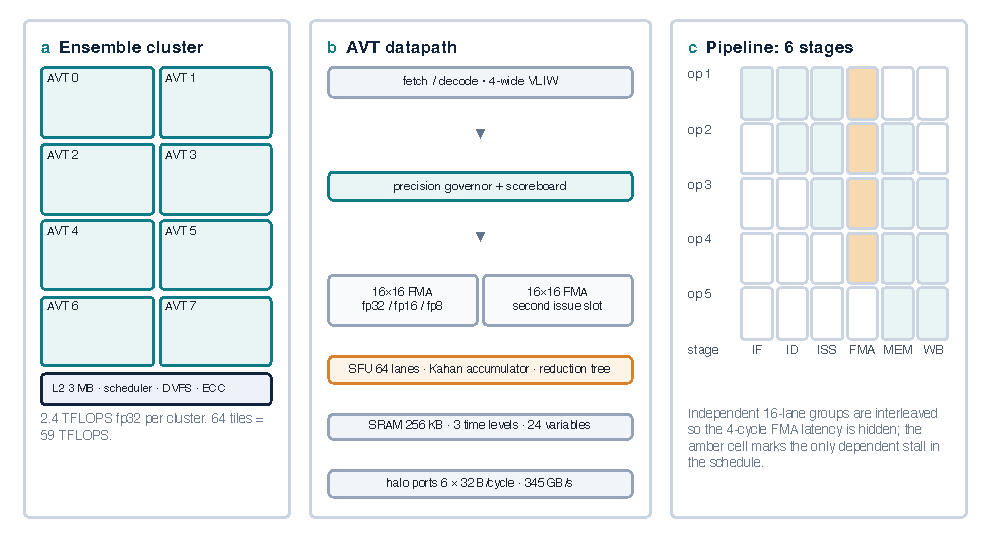
\includegraphics[width=\linewidth]{fig04_cluster}
\caption{Cluster and tile. (a) Eight AVTs share a 3 MB L2 slice, a scheduler and a DVFS domain.
(b) AVT datapath: decode, governor, two 16$\times$16 FMA blocks, SFU and Kahan reduction, SRAM and
halo ports. (c) Pipeline schedule; the amber cell is the only dependent stall in the schedule,
avoided by interleaving variables.}
\label{fig:avt}
\end{figure}

\subsection{Instruction set}
AVISA is a 64-bit, four-slot VLIW instruction set with ten opcodes (Table~\ref{tab:isa}). It is
not a general-purpose ISA: there are no branches, no indirect addressing, no floating-point
division, and no exception model beyond a sticky error flag. What it has instead are operations
that map one-to-one onto atmospheric kernels.

\begin{table}[t]
\centering\small
\caption{AVISA instruction set (excerpt). ``Slot cost'' is in lane-cycles for a 256-lane tile.}
\label{tab:isa}
\begin{tabular}{@{}lllr@{}}
\toprule
Opcode & Operation & Semantics & Slot cost\\
\midrule
\code{0x01} & \code{FMA.TILE} & $d = a\cdot b + c$ over 256 lanes & 1\\
\code{0x08} & \code{STENCIL3D} & 7-point operator with fused halo & 7\\
\code{0x10} & \code{ADVECT.SL} & 8-point semi-Lagrangian gather & 16\\
\code{0x14} & \code{ENS.SPREAD} & reduce 256 lanes to mean, $\sigma$, min, max & 9\\
\code{0x18} & \code{ENS.TL} & twin-trajectory tangent step & 2\\
\code{0x1c} & \code{DA.GAIN} & 16$\times$16 symmetric solve & 38\\
\code{0x20} & \code{PHYS.SAT} & saturation adjustment (Clausius--Clapeyron) & 1 SFU\\
\code{0x24} & \code{RNG.PHILOX} & counter-based random draw & 1 per 4 draws\\
\code{0x28} & \code{REDUCE.CONS} & mass and energy residual & 12\\
\code{0x2c} & \code{PREC.SET} & tile precision mode & 14\\
\bottomrule
\end{tabular}
\end{table}

A \code{STENCIL3D} retires 7 loads, 7 multiply--adds and a halo exchange that would take 19
instructions on a SIMT machine. More importantly it has a fixed, compiler-known latency, which is
what makes the per-tile cycle count (61,900 for the W1 step) a static number rather than a
statistical one.

\begin{figure}[t]
\centering
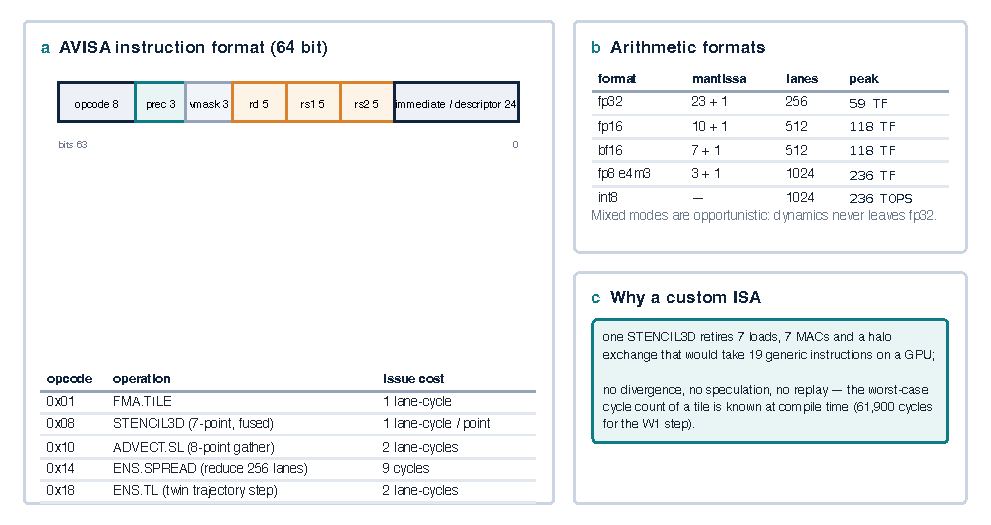
\includegraphics[width=\linewidth]{fig09_isa}
\caption{Instruction format and arithmetic modes. (a) 64-bit encoding with an 8-bit opcode, a
3-bit precision field and a 24-bit descriptor for stencil coefficients and halo offsets; (b)
supported formats and peak rates; (c) the argument for a custom ISA.}
\label{fig:isa}
\end{figure}

\subsection{Chaos monitor}
The monitor is a small block per cluster (7.2 mm$^2$ in total) that maintains a shadow trajectory
per tile, advanced with the same model but perturbed by one unit in the last place. Once per
kernel it computes the local finite-time Lyapunov estimate,
\begin{equation}
\lambda_i(t) = \frac{1}{\Delta t}\ln\frac{\|\delta_i(t+\Delta t)\|}{\|\delta_i(t)\|},
\end{equation}
and the ensemble spread $\sigma_i$ across the 256 lanes. Both are produced by \code{ENS.TL} and
\code{ENS.SPREAD}; the monitor costs 8\% of the tile area and 3.4\% of the step cycles. In return
the runtime gets a live predictability map, which drives the precision governor and gives the
forecast product a per-grid-cell confidence field at no extra cost.

The measured Lyapunov spectrum (Fig.~\ref{fig:req}(b)) has 11 positive exponents out of the 12
computed, consistent with the extensive chaos expected of Lorenz--96 at $F=8$. The leading
exponent, 0.34 day$^{-1}$, sets the horizon over which the precision argument of
Section~\ref{sec:precision} is valid.

\subsection{Ensemble analysis engine}
Each cluster carries a small dense-linear-algebra unit for the analysis phase: a 16$\times$16
symmetric eigensolver (cyclic Jacobi, fixed 38-cycle schedule), a rank-one update datapath and a
localisation multiplier. The unit executes the ensemble transform at 47.2 TFLOPS across the chip,
which is 40\% of the fp16 peak --- deliberately not a tensor-core-class engine, because analysis
is half of the daily arithmetic but only 6\% of the daily energy (Section~\ref{sec:results}).

The engine is what makes the honest comparison of Section~\ref{sec:results} possible: the H100 is
3.8$\times$ faster at dense analysis (3.8 s against 27.9 s) because it has tensor cores, and
\ac{1} still uses 4.4$\times$ less energy. A machine designed only for the forecast would have
looked better on the first number and worse on the second.

\subsection{Stochastic physics and conservation}
Stochastic perturbations (SPPT and SKEB) need fast, reproducible random numbers. Each tile has a
Philox-4$\times$32-10 generator in counter mode: the sequence is a pure function of (member, tile,
step, stream), so a run is reproducible from four integers and no generator state is stored.
Throughput is four draws per lane-cycle, enough for 76 stochastic draws per cell per step at 6\%
of the tile's issue budget.

A conservation monitor accumulates mass and energy residuals per tile and per step with
\code{REDUCE.CONS}, and reports them on a dedicated bus. Residuals above $10^{-9}$ relative trigger
a shadow fix-up pass every 64 steps. In the numerical experiment of Section~\ref{sec:validation}
the fp32 conservative advection drifts by $1.1\times10^{-8}$ per 1,200 steps without correction,
and by $3\times10^{-15}$ with fp64; the monitor is sized to catch the former before it matters.

\subsection{Reliability, availability and determinism}
All SRAM and L3 arrays carry SEC-DED ECC; the HBM links carry on-die ECC plus a link CRC; the
halo fabric has a per-flit parity check with replay. The arrays are scrubbed every 24 hours. With
1.41 Gbit of SRAM, a soft-error rate of $2\times10^{-3}$ FIT/bit and SEC-DED, the correctable rate
is 2.8 M FIT and the residual uncorrectable rate after scrubbing is below 300 FIT --- acceptable
for a data-centre part and two orders of magnitude below the memory-system FIT of the HBM stacks.

Reductions use a fixed tree with a compile-time order, there are no atomics in the numerical path,
and the RNG is counter-based. Two runs of the same binary on the same input produce bit-identical
output, which is a requirement for operational audit and for the reproducibility claims in
Section~\ref{sec:validation}.
